\section{Classification Approach Introduction}\label{sec:swing_control_class}

\begin{figure*}[t]
\centering
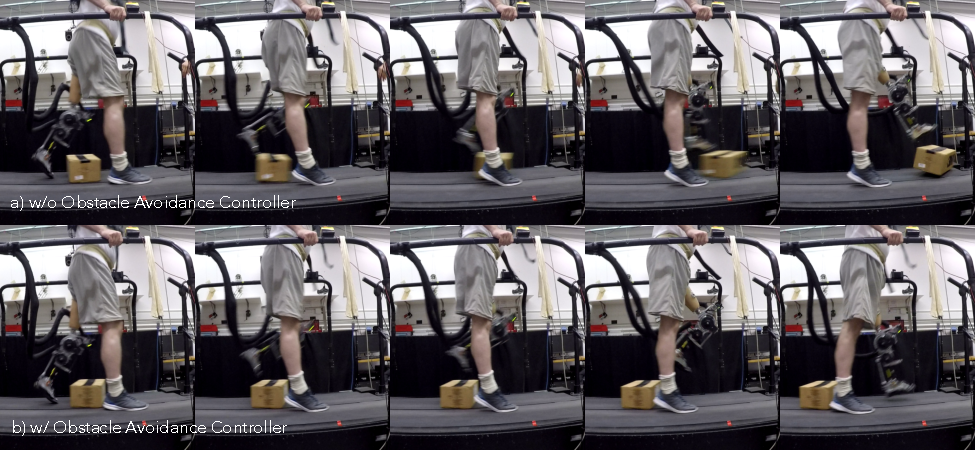
\includegraphics[width=\textwidth]{avoid_frames}
\caption{a)~Utilizing minimum jerk trajectories during swing does not allow for
appropriate adaptation of swing trajectories to enable obstacle avoidance.
b)~Our adaptive system learns online to detect the presence of an obstacle from
the amputee's late stance/early swing movements. Once detected, the controller
modifies the trajectories of the knee and ankle to achieve improved obstacle
clearance.}
\label{fig:avoid_frames}
\end{figure*}

Avoiding obstacles on the ground is a necessity for maintaining safety while
performing a variety of locomotion tasks. This behavior requires anticipation of
an obstacle and active leg control strategies to avoid it \citep{patla1995role}.
Transfemoral amputees, however, have a compromised ability to negotiate
obstacles, as shown in \Cref{fig:avoid_frames}, as current prosthesis technology
relies on mechanically passive knees that necessitate significant compensation
at the hip in order to replicate able-bodied trip recovery strategies
\citep{shirota2015transfemoral}. Compromised ability to avoid and recover from
trips may contribute to the large number of falls that leg amputees suffer. For
instance, 58\% of unilateral amputees reported a fall within a year
\citep{kulkarni1996falls}. Moreover, the fear of falling can cause amputees to
avoid activity, leading to further deterioration of their physical condition
\citep{miller2001prevalence}.

An increasing availability of powered prostheses in research labs provides the
opportunity to study active obstacle avoidance strategies in prosthetics,
although so far only a limited number of studies exist on this topic. These
studies focus on detecting and classifying the correct response strategy after
the amputee has tripped. For example, \citet{lawson2010stumble} developed a
classifier that uses fast Fourier transform and the root mean square of
accelerometer data as features to classify stumbles and recovery strategies,
respectively. \citet{zhang2011towards} found that adding EMG signals from the
residual limb to accelerometer data can help reduce false positives for stumble
and strategy detection. Finally, \citet{shirota2014recovery} identified the
optimal sliding window lengths and increments for feature calculation for trip
detection and strategy selection classifiers. While detecting and classifying
trip recovery strategies after their occurrence is a necessary step towards
obstacle avoidance, it does not provide a proactive prosthesis control strategy
that prevents obstacle encounters in the first place.

Another major drawback of the previous studies is that they train and test the
classifiers offline. However, a deployed trip classifier needs to function
online and deal with temporal adaptation of the learner and amputee. The
adaptation is required as the obstacle avoidance behavior triggered by a trip
classifier alters the amputee's movements and, therefore, the data used to train
the classifier. Consequently, trip classifiers trained offline may be
ineffective due to the mismatch of training and testing data, a common problem
faced in imitation and reinforcement learning \citep{ross2011reduction}. 

Here we present the first pilot study that combines online learning and
proactive control of a powered transfemoral prosthesis to implement obstacle
avoidance in amputee locomotion. The obstacle avoidance system uses early-swing
measurements of the residual limb angle, angular velocity, and linear
acceleration to recognize in-process obstacle avoidance attempts. To address the
online learning aspect of this system, we adapted a previously proposed
algorithm for detecting gait modes \citep{spanias2018online}. We also changed
the existing swing leg behavior of the prosthesis to facilitate obstacle
avoidance. This change includes a regression to predict the appropriate degree
of knee and ankle flexion given the user's previous obstacle response motions.
Finally, we evaluated the system behavior in trials with both non-amputee and
amputee subjects.
